\documentclass[11pt]{article}
\usepackage[a4paper,margin=1in]{geometry}
\usepackage{amsmath,amssymb,amsthm,mathtools}
\usepackage{booktabs}
\usepackage{enumitem}
\usepackage{float}
\usepackage{graphicx}
\usepackage{hyperref}
\usepackage[nameinlink,capitalise]{cleveref}
\usepackage[numbers,sort&compress]{natbib}

\newtheorem{theorem}{Theorem}[section]
\newtheorem{proposition}[theorem]{Proposition}
\newtheorem{corollary}[theorem]{Corollary}
\newtheorem{remark}[theorem]{Remark}
\theoremstyle{definition}
\newtheorem{definition}[theorem]{Definition}
\newcommand{\norm}[1]{\left\lVert#1\right\rVert}

\title{An Adaptive Upper--Lower Certificate Portfolio for Directional
Stein Tails\\
\large Safe Pareto Pruning, Three-Way Triage, and a Candidate Stage A1 Ledger}
\author{Liang Wang}
\date{July 2026}

\begin{document}
\maketitle

\begin{abstract}
RH-60--RH-68 produced several valid but incomparable tail mechanisms:
finite phase fusion, geometric completion, block Krylov centers,
physical-covariance PSD envelopes, weighted terminal residuals, and
phase-coherence lower bounds.  No single mechanism is uniformly best, and
RH-68 proves that a universal fixed-depth block rule is impossible.  This
paper assembles the mechanisms into an adaptive certificate portfolio while
preserving each input's claim level.

A candidate consists of a valid upper $U_c$ and a nonnegative cost vector
$b_c$ containing such entries as horizon, block depth, covariance focus, and
global PSD size.  We prove that Pareto-dominated candidates may be discarded
without changing any monotone budget decision.  The surviving portfolio has
three statuses: green when an upper meets every displayed budget, red when no
upper closes and a certified lower bound excludes the stated approximation
class, and amber otherwise.  A lower bound is never used to reject a broader
class than it proves.

For an exact finite prefix $F_L$ and any valid tail candidate,
\[
 \mathcal E\le F_L+U_c,
 \qquad
 \mathcal E\le F_L+\min_{c\in\mathcal C_L}U_c.
\]
This yields a conditional Stage A1 ledger: polylogarithmic finite terms,
tail uppers, and admissible cost entries imply the required
polylogarithmic Hardy bound.  The physical assumptions remain unproved.

On the archived RH-60 five-scale family, a one-percent selector grows from
horizon $4$ to $32$ and then remains at $32$.  At $\sigma=0.01$, RH-61's geometric
horizons are $1111$ and $307$, compared with phase horizon $32$.  The
covariance branch selects no focusing for the generic chain and complex-phase
models, but selects $\varepsilon=10^{-24}$ for exact cancellation, with
physical/global gains $1.001027/489.96$.  Exact and jittered Fourier rings are
red; wide phase arcs remain amber when only numerical misses, not analytic
lower bounds, are available.  A 256-bit Arb audit certifies one exact branch
of each type.  The architecture is now explicit, but the physical rows are
still binary64 diagnostics and Stage A1 is not closed.  No arithmetic trace
formula or Hilbert--Polya conclusion is claimed.
\end{abstract}

\noindent\textbf{Keywords:} certificate portfolio; Pareto frontier;
upper--lower bound; Stein tail; block Krylov method; phase-aware fusion.

\medskip
\noindent\textbf{MSC 2020:} 47A10; 47B65; 65F35; 90C29; 93B07.

\section{Introduction}

The route from RH-50 to RH-68 has become a collection of local theorems
rather than one monolithic estimate.  This is not a defect.  The physical
family can be phase-compressed at one scale, nonnormal at another, and close
to an exact cancellation ray at a third.  RH-68 shows that selecting one
fixed Krylov depth from stability data alone is mathematically impossible
\citep{WangDepthBarrier2026}.

The natural replacement is a portfolio.  Multicriteria Pareto reduction is
standard \citep{Ehrgott2005}, but a proof-oriented portfolio must also keep
upper and lower claims separate.  A failed upper is not a no-go theorem, and
a lower bound for one projection class does not rule out finite phase fusion
or a different packetization.

\subsection*{Contributions and boundary}

\begin{enumerate}[leftmargin=2.2em]
 \item We formalize safe dominance and Pareto pruning for rigorous upper
       candidates with vector-valued costs.
 \item We prove a green/red/amber triage rule that does not overextend lower
       bounds.
 \item We compose exact finite-prefix and terminal-tail certificates and give
       a conditional polylogarithmic budget theorem.
 \item We apply the ledger to archived physical and synthetic rows from
       RH-60, RH-61, RH-67, and RH-68.
\end{enumerate}

The portfolio logic is analytic.  A row is only as rigorous as its source;
binary64 physical diagnostics remain binary64 after selection.

\section{Certificate candidates and safe Pareto pruning}
\label{sec:pareto}

Let $\mathcal C$ be a finite family of candidates.  Candidate $c$ has a
nonnegative upper $U_c$ and a cost vector
\begin{equation}
 b_c=(b_{c,1},\ldots,b_{c,s})\in[0,\infty)^s.
 \label{eq:candidate}
\end{equation}
The coordinates may record horizon, block depth, covariance focus exponent,
metric conditioning, global PSD gain, or interval precision.  They must be
defined consistently within one comparison.

\begin{definition}
Candidate $c$ dominates $d$ if
\begin{equation}
 U_c\le U_d,qquad b_{c,j}\le b_{d,j}\quad(1\le j\le s),
 \label{eq:dominance}
\end{equation}
and at least one inequality is strict.  The Pareto frontier
$\mathcal P(\mathcal C)$ contains the undominated candidates.
\end{definition}

\begin{theorem}[Safe Pareto pruning]
\label{thm:pareto}
Let $\Phi(U,b)$ be nondecreasing in every coordinate.  Then
\begin{equation}
 \min_{c\in\mathcal C}\Phi(U_c,b_c)
 =\min_{c\in\mathcal P(\mathcal C)}\Phi(U_c,b_c).
 \label{eq:pareto-safe}
\end{equation}
Likewise, for any upper target and coordinatewise cost budgets, a feasible
candidate exists in $\mathcal C$ if and only if one exists on the frontier.
\end{theorem}

\begin{proof}
Every removed candidate is dominated by another candidate with no larger
objective value and no larger budget entries.  Repeating along the finite
dominance relation reaches an undominated candidate.
\end{proof}

The theorem is intentionally modest.  It does not average incomparable
certificates or convert diagnostics into validated uppers.

\section{Green, red, and amber}
\label{sec:triage}

Fix an upper target $\tau$, cost budgets $B_j$, and, when available, a lower
bound $\ell$ for a specifically named approximation error with target
$\delta$.

\begin{definition}[Three-way triage]
\label{def:triage}
The ledger status is:
\begin{enumerate}[leftmargin=2.2em]
 \item \emph{green} if some valid upper candidate has
       $U_c\le\tau$ and $b_{c,j}\le B_j$ for every $j$;
 \item \emph{red for the stated approximation class} if no candidate is green
       and a certified lower bound satisfies $\ell>\delta$;
 \item \emph{amber} otherwise.
\end{enumerate}
\end{definition}

\begin{proposition}[Triage soundness]
\label{prop:triage}
A green status proves the displayed upper budget.  A red status proves only
that the class named by $\ell$ misses its displayed approximation target.
An amber status makes neither assertion.
\end{proposition}

\begin{proof}
Green is the definition of a valid feasible upper.  Red is the contradiction
between a certified lower bound and the target for the same quantity.  No
logical conclusion follows when neither condition holds.
\end{proof}

This discipline matters for the phase arcs in RH-68.  A binary64 depth miss
is evidence, not an analytic lower bound, so wide arcs are amber rather than
red.

\section{Finite-prefix and tail composition}
\label{sec:composition}

Suppose an exact finite response calculation and a positive tail mechanism
give, for every admissible candidate $c$ at horizon $L$,
\begin{equation}
 \mathcal E\le F_L+U_{L,c}.
 \label{eq:prefix-tail}
\end{equation}
This includes the RH-60 phase-aware finite Gram followed by a geometric,
block, or weighted residual completion \citep{WangPhaseTail2026}.

\begin{theorem}[Adaptive composition]
\label{thm:composition}
For every horizon $L$,
\begin{equation}
 \mathcal E\le F_L+min_{c\in\mathcal C_L}U_{L,c},
 \label{eq:adaptive-upper}
\end{equation}
and the minimum may be restricted to the Pareto frontier.  Taking a further
minimum over a finite set of horizons remains valid.
\end{theorem}

\begin{proof}
Equation \eqref{eq:prefix-tail} holds separately for every candidate.  Taking
the minimum of right sides preserves the inequality; \cref{thm:pareto}
removes only dominated entries.
\end{proof}

\begin{corollary}[Conditional polylogarithmic ledger]
\label{cor:conditional}
Let $\sigma\downarrow0$.  Suppose there exist selected horizons and
candidates such that
\begin{equation}
 F_{L_\sigma}=O(\log(1/\sigma)^a),
 \qquad
 U_{L_\sigma,c_\sigma}=O(\log(1/\sigma)^b),
 \label{eq:polylog-upper}
\end{equation}
and every analytically relevant transfer cost in $b_{c_\sigma}$ is
polylogarithmic.  Then the corresponding directional Hardy energy is
polylogarithmically bounded and can be inserted into the conditional RH-50
bridge.
\end{corollary}

\begin{proof}
Apply \eqref{eq:prefix-tail} and add the two polylogarithmic quantities.  The
remaining transfer factors are covered by the stated cost assumption.
\end{proof}

The corollary is a bookkeeping theorem, not Stage A1: none of its physical
uniformity hypotheses is proved here.

\section{Portfolio audit}
\label{sec:audit}

\subsection{Archived physical horizon branch}

For every RH-60 row and side, candidates are the stored horizons
$\{0,1,2,4,8,16,32,64\}$.  The upper entry is phase-aware completion divided
by the archived exact Hardy energy; the cost is horizon.  We select the least
horizon with gain at most $1.01$ and compare it with RH-61's packetwise
geometric horizon for the same tolerance.

\begin{table}[H]
\centering
\caption{One-percent horizon portfolio.}
\label{tab:physical}
\begin{tabular}{rrrrrr}
\toprule
$\sigma$ & phase L/R & geometric L/R & saving left & saving right\\
\midrule
0.16 & 4/4   & 8/9     & 2.00 & 2.25\\
0.08 & 8/8   & 22/24   & 2.75 & 3.00\\
0.04 & 16/16 & 67/69   & 4.19 & 4.31\\
0.02 & 32/32 & 220/165 & 6.88 & 5.16\\
0.01 & 32/32 & 1111/307& 34.72& 9.59\\
\bottomrule
\end{tabular}
\end{table}

The selection is deterministic over archived binary64 values.  It is not an
interval-certified physical upper and does not establish an asymptotic
horizon law.

\subsection{Covariance and depth branches}

The RH-67 covariance frontier uses physical gain as upper and
$(\text{focus exponent},\text{global gain})$ as costs
\citep{WangCovarianceEnvelope2026}.  Targets $4.0$ and $1.3$ select isotropic
covariance for the nonnormal chain and complex-phase model.  The exact
cancellation target $1.01$ selects $\varepsilon=10^{-24}$, physical gain
$1.001027$, focus exponent $24$, and global gain $489.96$.

The RH-68 exact rings and all four jittered rings are red at the displayed
depth budgets: their spectral lower bounds at horizon and depth $32$ range
from $0.97848$ to $1$, above the $0.1$ target.  For phase arcs and depth budget
$8$, widths $0,0.03,0.1,0.3$ are diagnostic green; widths $1,3,2\pi$ are
amber, because the archive contains misses but no analytic lower bound for
those particular arcs.

\begin{figure}[H]
\centering
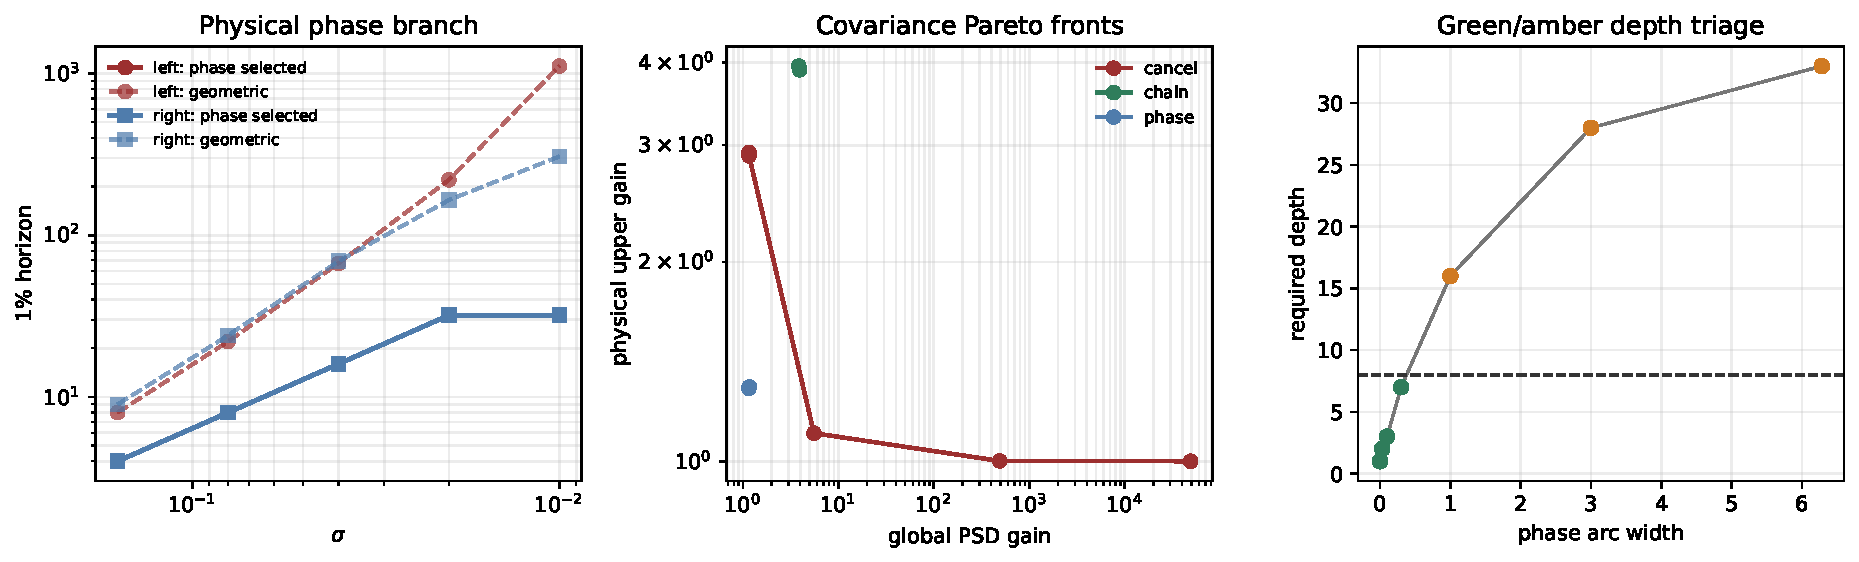
\includegraphics[width=0.99\textwidth]{figures/adaptive_certificate_portfolio.pdf}
\caption{Left: phase fusion versus geometric horizons.  Middle: covariance
Pareto fronts.  Right: green and amber arc-depth decisions under budget
$k\le8$.}
\label{fig:portfolio}
\end{figure}

A 256-bit Arb audit exercises three exact branches.  It certifies that
$q=0.99$ first reaches $10^{-3}$ at horizon $688$, that the focused exact
cancellation candidate has physical gain below $1.01$ and global gain below
$500$, and that the exact Fourier lower bound $1$ rejects a ten-percent
projection target.

\section{Route consequence}
\label{sec:route}

The candidate architecture is now explicit:
\begin{equation}
 \begin{aligned}
 \text{finite phase fusion}
 &\longrightarrow \text{depth lower gate}
 \longrightarrow \text{block/covariance upper}\\
 &\longrightarrow \text{weighted terminal residual}
 \longrightarrow \text{Pareto selection}.
 \end{aligned}
 \label{eq:architecture}
\end{equation}

RH-70 should apply this ledger to a finite production family with outward
rounding.  The purpose is not yet a continuum theorem.  It is to determine,
without optimistic binary64 substitutions, whether each physical row is
green, red for a specific route, or honestly amber.  That audit will decide
which asymptotic theorem is worth attempting next.

\section{No arithmetic or Hilbert--Polya conclusion}

This paper constructs no self-adjoint operator, no $T\log T$ counting law,
no prime-power trace formula, and no completed-zeta identity.  It makes no
Hilbert--Polya or Riemann-hypothesis claim.  Stage A1 and unconditional Stage
A4 remain open.

\section{Reproducibility}

The directory contains portfolio logic, tests, archived-input composition,
an Arb audit, figures, hashes, and publication artifacts.  The main commands
are:
\begin{verbatim}
pytest -q -p no:cacheprovider
python experiments/run_certificate_portfolio.py
python experiments/run_arb_portfolio_audit.py
MPLBACKEND=Agg python experiments/make_figures.py
latexmk -pdf -interaction=nonstopmode -halt-on-error main.tex
\end{verbatim}

The Pareto, triage, and composition statements are analytic.  Physical
phase rows and generic covariance rows retain their binary64 source status.
Production interval validation, a physical covariance theorem, asymptotic
phase compression, Stage A1, unconditional Stage A4, a self-adjoint
Hilbert--Polya operator, an arithmetic trace formula, and a zeta-zero identity
remain open.

\bibliographystyle{plainnat}
\bibliography{references}
\end{document}
